\documentclass[runningheads]{llncs}
\usepackage[T1]{fontenc}
\usepackage{amsmath,amssymb,booktabs,graphicx}
\usepackage{xcolor}
\usepackage{pgfplots}
\pgfplotsset{compat=1.18}
% Placeholder marker for values that are NOT in the log or the original
% manuscript. Every \tbd must be filled from the analysis output (or the
% sentence removed) before submission. (R3: no \tbd is used.)
\newcommand{\tbd}{\textcolor{red}{\textbf{[TBD]}}}

\begin{document}
\title{Measuring AI-Relatedness in Multilingual Public Procurement Notices: Dictionary-Based Screening, Embedding Classifiers, and Design-Based Inference}
\titlerunning{Measuring AI-Relatedness in Multilingual Procurement Notices}
\author{Jinkyu Lee\orcidID{0000-0002-0886-1572} \and Chang Soo Sung\thanks{Corresponding author.}\orcidID{0000-0001-9284-817X}}
\authorrunning{J. Lee and C. S. Sung}
\institute{Department of Technology Entrepreneurship, Graduate School, Dongguk University, Seoul, Republic of Korea\\ \email{leejinkyu0612@naver.com, redsun44@dgu.ac.kr}}
\maketitle

\begin{abstract}
English keyword lists are a common way to identify AI-related text, but their error in multilingual procurement data and its downstream consequences are seldom quantified. Among 54,160 IT and software award notices in Tenders Electronic Daily (TED), 2024--2025 (6.1\% in English), we compared scalable methods against a stratified probability sample of 1,199 notices annotated with a fixed codebook by a primary large language model (LLM) and compared with a second LLM (design-weighted $\kappa=0.77$); without expert validation, all estimands are relative to this LLM reference. A multilingual dictionary achieved the highest observed F1 (0.63, 95\% CI 0.50--0.78) and doubled the recall of the English dictionary (0.56 vs.\ 0.28). Design-weighted embedding and TF-IDF classifiers scored F1 0.06 and 0.10 at a fixed 0.5 threshold (0.34--0.36 post hoc for the embedding classifier with threshold tuning or unweighted training). The estimated reference-defined prevalence was 2.32\% with design-based supervised learning (DSL; CI 1.56--3.21\%) and 2.06\% with Horvitz--Thompson estimation (CI 1.38--2.94\%), versus a 0.83\% English-dictionary flag rate; the excess remained positive under alternative references and cross-fitting schemes, but its size depended on four heavily weighted labels. A plug-in regression using the multilingual dictionary suggested that AI-related notices were 4.9 percentage points less likely to report a single tender, but DSL did not establish the sign of this association because its moment matrix became indefinite under full controls. Keyword-based AI indicators need multilingual terms and quantified measurement error.\keywords{Public procurement \and AI-relatedness \and Multilingual text classification \and Design-based supervised learning \and Measurement error \and LLM annotation.}
\end{abstract}

%======================================================================
\section{Introduction}
Public procurement is a principal channel through which governments acquire artificial intelligence (AI) systems and services \cite{hickok2022}, and quantifying this market requires deciding which procurement notices concern AI. Text-based measures of AI demand and investment typically use English job postings and r\'esum\'es, with predefined AI skill lists \cite{acemoglu2022} or data-driven skill measures \cite{babina2024}; for procurement notices, an English keyword list is the natural transfer. Such lists are transparent and cheap, but their accuracy is seldom reported against a reference annotation, and their error is rarely carried into the analyses that use them.

Two features of procurement data make this omission consequential. First, notices in Tenders Electronic Daily (TED) may be published in any of the 24 official EU languages \cite{ahmia2018}; of the 54,160 IT and software award notices analysed here, only 6.1\% were in English, so an English dictionary may miss AI purchases in a language-dependent way. Second, a text-based AI indicator is often used as a regressor in a second-stage analysis, and plugging machine-generated variables into regressions can yield biased estimates and invalid confidence intervals unless the measurement error is addressed \cite{battaglia2025,egami2023}; correction methods also differ in finite samples \cite{audinet2025}.

We therefore examine how the measurement of AI-relatedness affects classification accuracy, the share of AI-related notices, and the association between AI-relatedness and single bidding, a standard indicator of weak competition \cite{fazekas2016}. Six methods---two keyword dictionaries, zero-shot natural language inference (NLI), an embedding-prototype score, and two supervised classifiers---are compared against a codebook-based reference annotation of a stratified probability sample, and design-based supervised learning (DSL) \cite{egami2023} and Horvitz--Thompson (HT) estimation are applied under hypotheses fixed before annotation. No human expert labels were available: the reference labels come from an LLM, compared with a second LLM and selectively re-adjudicated by a third, so all estimands are defined relative to this reference, and all influential cases are disclosed.

This methodological case study contributes (i) a design-based, language-stratified evaluation of AI-relatedness measurement in multilingual procurement notices; (ii) an assessment of how prevalence estimates depend on the estimator, the cross-fitting scheme, and a few contested, heavily weighted reference labels; and (iii) an analysis of how measurement uncertainty propagates into competition estimates, with a scale-invariant diagnostic that locates when DSL regression becomes uninformative. No new learning algorithm is proposed.

%======================================================================
\section{Related Work}
\subsubsection{Text-based measurement of AI demand.} Beyond the vacancy- and r\'esum\'e-based measures above \cite{acemoglu2022,babina2024}, LLMs have been used to score occupational exposure to AI \cite{eloundou2024}. Text-as-data surveys stress that dictionary and supervised measures trade transparency against recall and that their error should be quantified \cite{gentzkow2019}; these studies mainly analyse English text.

\subsubsection{Procurement analytics.} TED data support multilingual corpora \cite{ahmia2018} and national award databases \cite{potin2023}, and single bidding is widely used to assess competition and integrity risk \cite{fazekas2016,decarolis2022}. We are not aware of work that quantifies the error of keyword screening for technology purchases across languages with a probability sample, or that traces this error into competition estimates.

\subsubsection{LLM annotation and inference with predicted variables.} LLMs can match or exceed crowd workers on several annotation tasks \cite{gilardi2023}, but performance varies widely across tasks \cite{ziems2024}, and agreement between LLMs does not establish accuracy because models can share errors. Prediction-powered inference \cite{angelopoulos2023} and DSL \cite{egami2023} combine a small labelled sample with abundant predictions for asymptotically valid estimates. Multilingual encoders \cite{wang2024me5,reimers2020} and NLI-based zero-shot classification \cite{yin2019,he2023} are alternatives to dictionaries whose performance varies by task and language \cite{muennighoff2023}.

%======================================================================
\section{Method}
\subsection{Problem Formulation}
Let $i=1,\dots,N$ index award notices (not contracts) in the analysis frame, one per TED publication number. Let $X_i^*$ denote the latent AI-relatedness of notice $i$ and $X_i\in\{0,1\}$ its reference label, i.e., AI-relatedness as operationalised by the primary LLM under a fixed codebook (Sect.~\ref{sec:ref}). $X_i$ is observed only for a labelled subsample $\mathcal{L}$ drawn with known inclusion probabilities $\pi_i$; for every notice, a method $m$ produces a prediction $\hat{X}^m_i$ or a score. All design-based estimands target $X$, not $X^*$: (a) the accuracy of each method relative to $X$, (b) the reference-defined prevalence $\theta=N^{-1}\sum_i X_i$, and (c) the coefficient $\beta$ on $X_i$ in a model of single bidding $Y_i$ with controls $W_i$ on the regression subpopulation of Sect.~\ref{sec:data}. DSL and HT correct the errors of $\hat{X}^m$ relative to $X$; errors of $X$ relative to $X^*$ are not corrected.

\subsection{Construct and Reference Annotation}
\label{sec:ref}
A notice is AI-related if the procured object includes the development, supply, licensing, operation, or consulting and training on a system whose core functionality relies on AI techniques (machine learning, deep learning, natural language processing or LLMs, chatbots, computer vision, speech recognition or synthesis, or predictive models learned from data). Generic software, workflow automation without AI, dashboards without learning components, and hardware are coded as not AI-related. Each sampled notice was annotated by a primary LLM (Claude Haiku 5.5) and a secondary LLM (Gemini 2.5 Flash-Lite) with the same zero-shot prompt (temperature 0, JSON output). The pre-specified reference is the primary label $X$; unparsable responses are treated as missing, never as negative. Two pre-specified variants require agreement of both annotators (available-label intersection $X_\wedge$) or either annotator (available-label union $X_\vee$); both fall back to the primary label for the 33 notices without a secondary label. Post hoc, a third LLM (DeepSeek-Chat-v3.1) re-annotated with the same prompt the 123 notices whose first two labels disagreed or lacked a secondary label, plus all primary positives in strata C and D; the \emph{selectively adjudicated reference} $X_{\mathrm{adj}}$ takes the majority of the available labels, and all other notices keep the primary label. These are cross-model agreement and sensitivity assessments, not independent validation; all influential cases are therefore disclosed (Table~\ref{tab:cases}).

\subsection{Measurement Methods}
\textbf{M1} is an English AI dictionary (22 patterns, e.g., \textit{machine learning}, \textit{chatbot}). \textbf{M2} adds core equivalents of \textit{artificial intelligence}, \textit{machine learning}, \textit{neural network}, \textit{language model}, and \textit{chatbot} in the EU languages and the abbreviations KI and IA. Because M1 and M2 define the sampling strata, both were fixed before sampling and annotation; since M2 also changes the term set, their comparison reflects multilingual coverage and term choice jointly, not a pure language effect. \textbf{M3} is zero-shot NLI with mDeBERTa-v3-base-mnli-xnli \cite{he2023,yin2019} and the hypothesis ``This procurement is about artificial intelligence'' (entailment probability $\ge 0.5$); it is label-free. \textbf{M4} is the maximum cosine similarity between a notice and five English prototype queries in the multilingual-e5-small space \cite{wang2024me5}; the score is label-free, but its threshold is selected within training folds, and its English prototypes make it not language-neutral. \textbf{M5}, the pre-specified embedding-based classifier, is an $L_2$-regularised logistic regression on multilingual-e5-small embeddings trained on the reference labels with weights $1/\pi_i$ and a fixed threshold of 0.5. \textbf{M6} replaces the embeddings with character 3--5-gram TF-IDF features. All label-trained components, including thresholds and TF-IDF vocabularies, are cross-fitted: predictions for labelled notices come from five folds that exclude them; in the pre-specified implementation, unlabelled notices are scored by a model refitted on all labels. E5 inputs use the `passage:'/`query:' prefixes with mean pooling.

\subsection{Sampling Design and Design-Based Estimation}
\label{sec:design}
Because AI notices are rare, the frame was stratified: A (M1 hit), B (M2 hit but not M1), C (neither, but M4 similarity in the top 3\%), and D (remaining notices), and simple random samples were drawn without replacement within strata (seed 2027). As pre-specified, $\pi_h=n^{\mathrm{drawn}}_h/N_h$ and the one stratum-C notice without a parsable primary label is omitted (Table~\ref{tab:design}), which is equivalent to coding it 0; a weight $N_h/n_h$ (missing at random within the stratum) would give an estimate between codings 0 and 1. Accuracy metrics weight labelled notices by $1/\pi_i$. For prevalence and regression, DSL replaces the unobserved $X_i$ with the pseudo-outcome
\begin{equation}
\tilde{X}_i=\hat{g}(T_i)+\frac{R_i}{\pi_i}\bigl(X_i-\hat{g}(T_i)\bigr),
\label{eq:pseudo}
\end{equation}
where $\hat{g}$ is the cross-fitted M5 probability, $T_i$ the text, and $R_i$ the labelling indicator. For a fixed $\hat{g}$, $E_p(R_i)=\pi_i$ gives $E_p(\tilde{X}_i)=X_i$ under the sampling design, so $\hat\theta_{\mathrm{DSL}}=N^{-1}\sum_i\tilde{X}_i$ is design-unbiased under the stated sampling and response-weighting assumptions whatever the accuracy of $\hat{g}$, which affects only its variance. Under appropriate sampling and cross-fitting regularity conditions, DSL permits asymptotically valid inference without requiring a correctly specified auxiliary predictor \cite{egami2023}. The pre-specified implementation meets these conditions only approximately, because unlabelled notices are scored by a predictor trained on all labels. Post hoc, we therefore also cross-fitted $\hat{g}$ over the entire frame, scoring all notices of each of five folds with the model trained on the labelled notices outside that fold; under sampling without replacement a fold's predictor is still not exactly independent of its inclusion indicators, so we claim neither finite-sample unbiasedness nor exact asymptotic validity. Setting $\hat{g}\equiv0$ yields the HT estimator. If $\hat{g}=c_h$ within strata, $\hat\theta_{\mathrm{DSL}}-\hat\theta_{\mathrm{HT}}=N^{-1}\sum_h c_h(N_h-\sum_{i\in\mathcal{L}_h}\pi_i^{-1})=0$ for the M1 and M2 indicators (weights sum to $N_h$ except in stratum C, where both are 0); variance gains over HT require informative within-stratum predictions, chiefly in stratum D.

For the linear probability model $Y_i=\beta X_i+W_i^\top\gamma+\varepsilon_i$ on the regression sample $\mathcal{R}$ ($N_R$ notices), every OLS moment is linear in $X_i$ because $X_i^2=X_i$, so $\tilde{X}_i$ replaces $X_i$ wherever it appears:
\begin{equation}
\hat{A}=\frac{1}{N_R}\sum_{i\in\mathcal{R}}\begin{pmatrix}\tilde{X}_i & \tilde{X}_iW_i^\top\\ W_i\tilde{X}_i & W_iW_i^\top\end{pmatrix}\equiv\begin{pmatrix}a & c^\top\\ c & B\end{pmatrix},\quad
\hat{b}=\frac{1}{N_R}\sum_{i\in\mathcal{R}}\begin{pmatrix}\tilde{X}_iY_i\\ W_iY_i\end{pmatrix}\equiv\begin{pmatrix}d\\ e\end{pmatrix}.
\label{eq:moments}
\end{equation}
Solving $\hat{A}(\hat\beta,\hat\gamma^\top)^\top=\hat{b}$ by partitioned inversion,
\begin{equation}
\hat\beta=\frac{d-c^\top B^{-1}e}{S},\qquad S=a-c^\top B^{-1}c,
\label{eq:schur}
\end{equation}
where the Schur complement $S$ of $B$ is the information on AI-relatedness left after partialling out $W$. It is non-negative when $X$ is observed, but not in DSL: $a$ is linear in $\tilde{X}$, whereas $c^\top B^{-1}c=N_R^{-1}\lVert P_W\tilde{X}\rVert^2$ ($P_W$: projection onto $W$) is quadratic, so $\hat{A}$ can be indefinite. For fixed $\hat{g}$, $a$ and $c$ are design-unbiased, but $E_p(S)=S_X-\mathrm{tr}\{B^{-1}\mathrm{Var}_p(c)\}$, with $S_X$ the value under full observation of $X$; the downward bias grows with the number of controls and the variance of the pseudo-outcomes (a pseudo-outcome isolated in a fixed-effect cell of $n_c$ notices adds about $\tilde{X}_i^2/n_c$ to $\lVert P_W\tilde{X}\rVert^2$ but only $\tilde{X}_i$ to $N_Ra$). Unlike the condition number $\mathrm{cond}(\hat{A})$, $S$ is invariant to reparametrising $W$. Labelled notices in $\mathcal{R}$ keep their frame inclusion probabilities. Prevalence CIs are stratified bootstrap intervals; for regression we report sandwich standard errors and, for the pre-specified DSL estimate, a bootstrap interval. A linear probability model is used because the specification contains over 100 fixed effects, for which logit estimates are less stable.

%======================================================================
\section{Experimental Setup}
\subsection{Data}
\label{sec:data}
We retrieved all TED contract award notices (eForms type \texttt{can-standard}) published between 1 January 2024 and 31 December 2025 whose CPV classification falls under IT services (72000000) or software packages (48000000), using the public TED Search API v3 (reuse permitted by the European Commission's reuse policy). After deduplication by publication number (CPV matching includes additional CPV codes), 55,508 notices from 50 buyer countries in 23 languages remained; excluding notices with fewer than ten characters of title and description left an analysis frame of $N=54{,}160$, of which 3,308 (6.1\%) were in English. The text of a notice is its procedure title and description in its first official language (median 378 characters, truncated at 2,000). No personal data are used, and notice texts are not redistributed.

Of the 54,160 frame notices, 17,864 report no received-tenders count, 4,635 report more than one (lot-level counts in multi-lot notices), and 31,661 report exactly one. Because eForms records this count per lot result, a notice with one reported count need not concern a single lot. Excluding counts of zero (1,271; no tender, outside the single-bidding estimand) and above 100 (2; probable recording errors, cf.\ \cite{potin2023}) left a regression sample $\mathcal{R}$ of 30,388 notices (630 labelled). The outcome $Y_i$ indicates that the notice's single reported count of tenders (eForms received-submissions type `tenders', not the SME or electronic sub-counts) equals one; it is a notice-level proxy, and 46.2\% of $\mathcal{R}$ had $Y_i=1$. Design weights do not correct for selection into $\mathcal{R}$; post hoc, $\mathcal{R}$ contained fewer English notices than the 23,772 excluded notices (3.9\% vs.\ 9.0\%) but had similar flag rates (M1 0.82\% vs.\ 0.85\%; M2 1.55\% vs.\ 1.72\%). Controls are fixed effects for buyer country, CPV division (26 levels after pooling divisions with fewer than 30 notices; matching on additional codes admits divisions beyond the two retrieved), procedure type, buyer legal type, and publication quarter, plus log contract value with a missing-value indicator \cite{fazekas2016,decarolis2022}. Values are not converted between currencies, so country effects absorb currency only for single-currency countries.

\subsection{Sample, Annotation, and Implementation}
Table~\ref{tab:design} reports the sampling design. The 1,200 sampled notices were annotated by both LLMs through OpenRouter between 11:54 and 12:16 KST on 27 November 2026 (2,400 requests). The secondary model returned unparsable text for 86 notices; re-querying them with the same prompt and a 120-token output limit recovered 53, leaving 33 without a secondary label (17 in stratum D). Bootstrap CIs use 2,000 resamples drawn with replacement within strata of the labelled sample; classifiers and thresholds are not refitted within replicates, so these intervals approximate sampling uncertainty conditional on the realised predictions. Resampling with replacement omits the finite-population correction, which matters in strata A and B (sampling fractions 0.556 and 0.584) but little for prevalence, whose uncertainty stems almost entirely from stratum D (fraction below 0.01).

\begin{table}[t]
\caption{Stratified reference sample. $N_h$: frame notices; drawn: sampled notices; $n_h$: notices with a parsable primary label; $\pi_h=\mathrm{drawn}/N_h$ (for D, $450/51{,}756$); Pos.: notices coded AI-related by the primary annotator; Est.: weighted estimate of AI-related notices in the stratum.}\label{tab:design}
\centering
\begin{tabular}{llrrrrrr}
\toprule
Stratum & Definition & $N_h$ & Drawn & $n_h$ & $\pi_h$ & Pos. & Est. \\
\midrule
A & English-dictionary hit (M1) & 450 & 250 & 250 & 0.556 & 172 & 310 \\
B & Multilingual-dictionary hit only (M2) & 428 & 250 & 250 & 0.584 & 183 & 313 \\
C & No hit; M4 score in top 3\% & 1,526 & 250 & 249 & 0.164 & 5 & 31 \\
D & Remaining notices & 51,756 & 450 & 450 & 0.009 & 4 & 460 \\
\midrule
Total & & 54,160 & 1,200 & 1,199 & & 364 & 1,114 \\
\bottomrule
\end{tabular}
\end{table}

\subsection{Pre-specified Hypotheses and Testing}
The analysis plan was time-stamped in the project repository before reference annotation (commit 7314e8d, 27 November 2026, 11:12 KST; amendment commit b1eb797, 12:22 KST); it was not externally preregistered. It stated: \textbf{H1} the recall of M1 is lower for non-English than for English notices, i.e., $\Delta_{\mathrm{H1}}=R_{\mathrm{non}}-R_{\mathrm{EN}}<0$; \textbf{H2} M5 attains higher F1 than M1 (H2a) and M2 (H2b); \textbf{H3} the DSL prevalence exceeds the M1 prevalence; and \textbf{H4} the DSL coefficient on AI-relatedness in the single-bidding model differs from zero (two-sided). One-sided bootstrap $p$-values for the four tests H1, H2a, H2b, and H3 are Holm-adjusted as one family; H4 is assessed by its 95\% CI. All reported CIs are unadjusted 95\% intervals. One amendment, committed before the affected results were computed, restricted M3 to the labelled sample because its projected CPU time for the frame exceeded the plan's six-hour rule; M3 is therefore evaluated for accuracy only. All other analyses, including the re-query, adjudication, HT comparisons, ablations, diagnostics, leave-one-out (LOO) analyses, full-frame cross-fitting, and bootstrap refitting, are post hoc and support no confirmatory claim.

%======================================================================
\section{Results}
\subsection{Reference Annotation}
Among the 1,166 notices with both labels after the re-query, unweighted $\kappa$ was 0.92 and design-weighted $\kappa$ 0.77 (95\% CI 0.60--0.95); weighted positive and negative specific agreement were 0.78 and 0.996. Weighted $\kappa$ was lower for English (0.48) than for non-English notices (0.82); the unweighted--weighted gap reflects disagreement in the heavily weighted unflagged strata. Table~\ref{tab:cases} lists all nine primary positives in strata C and D. Each stratum-D notice carries a weight of about 115, so the four stratum-D positives account for 460 of the 1,114 estimated AI-related notices (41\%). $X_{\mathrm{adj}}$ retains two of the four stratum-D and four of the five stratum-C positives (359 positives in total).

\begin{table}[t]
\caption{All primary-reference positives in the unflagged strata C and D, with the labels of the secondary (S) and third (T) LLM and the selectively adjudicated reference $X_{\mathrm{adj}}$. Objects are paraphrased from the notice text. Post hoc.}\label{tab:cases}
\centering
\begin{tabular}{llllccc}
\toprule
Notice & Str. & Lang. & Procured object (paraphrased) & S & T & $X_{\mathrm{adj}}$ \\
\midrule
192940-2025 & C & ENG & Digital dictation and voice-recognition system & 1 & 1 & 1 \\
86787-2024  & C & ENG & Biometric authentication with facial recognition & 1 & 1 & 1 \\
327445-2025 & C & ENG & Operation and development of a statistical model & 0 & 0 & 0 \\
678350-2025 & C & SPA & Voice assistant for primary-care appointments & 1 & 1 & 1 \\
810556-2025 & C & ENG & Reseller services for Darktrace software & 1 & 1 & 1 \\
755854-2025 & D & SPA & Access to specialised genetics software & 0 & 0 & 0 \\
787623-2025 & D & RON & Integrated e-services platform and licences & 0 & 0 & 0 \\
500255-2024 & D & ENG & Train-running forecast information (TIS) & 0 & 1 & 1 \\
201930-2025 & D & CES & Support of a biometric face-detection system & 1 & 1 & 1 \\
\bottomrule
\end{tabular}
\end{table}

\subsection{Classification Accuracy (H1, H2)}
Table~\ref{tab:acc} reports design-weighted accuracy. M2 achieved the highest observed F1 (0.63, 95\% CI 0.50--0.78), doubling the recall of M1 (0.56 vs.\ 0.28) at similar observed precision (0.71 vs.\ 0.69); no test of M2 against the other methods was pre-specified. H1 was not supported under the primary reference: the recall of M1 was 0.25 for English and 0.28 for non-English notices ($\Delta_{\mathrm{H1}}=0.04$ from unrounded recalls, CI $-0.55$ to 0.27), largely because one English stratum-D positive carries a large weight. H2 was not supported, and the observed differences had the opposite sign: at the 0.5 threshold, M5 and M6 predicted almost no positives, although M5 had the highest AUPRC among pre-specified methods (0.33). The F1 differences M5$-$M1 ($-0.34$, CI $-0.45$ to $-0.26$) and M5$-$M2 ($-0.57$, CI $-0.70$ to $-0.45$) were negative (Holm-adjusted $p=1.00$ for both). In a post hoc $2\times2$ ablation, M5's F1 was 0.06 with training weights and threshold 0.5, 0.34 with weights and a fold-tuned threshold, 0.36 without weights at 0.5, and 0.35 without weights and with a tuned threshold (M5u), so the low F1 was sensitive to the combination of design-weighted training and the fixed 0.5 threshold; M5u remained below M2 (difference $-0.28$, CI $-0.39$ to $-0.18$). M2 retained the highest observed F1 under $X_{\mathrm{adj}}$, $X_\wedge$, and $X_\vee$ (F1 0.66, 0.73, 0.64), with a paraphrase-multilingual-MiniLM encoder (M5 F1 0.30), and for non-English notices (F1 0.40, 0.66, 0.05 for M1, M2, M5). $\Delta_{\mathrm{H1}}$ was $-0.32$ (CI $-0.61$ to $-0.06$) under $X_\wedge$ but 0.06 (CI $-0.61$ to 0.29) under $X_{\mathrm{adj}}$.

\begin{table}[t]
\caption{Design-weighted accuracy against the primary reference ($n=1{,}199$). R$_\mathrm{EN}$/R$_\mathrm{non}$: recall for English/non-English notices. AUPRC only for score-based methods. $^\S$Labelled sample only (amendment); excluded from prevalence and regression. $^\dagger$Post hoc variant (unweighted training, fold-internal threshold), not part of the pre-specified tests.}\label{tab:acc}
\centering
\begin{tabular}{lrrrrrr}
\toprule
Method & Precision & Recall & R$_\mathrm{EN}$ & R$_\mathrm{non}$ & F1 [95\% CI] & AUPRC \\
\midrule
M1 English dictionary & 0.69 & 0.28 & 0.25 & 0.28 & 0.40 [0.30, 0.53] & -- \\
M2 Multilingual dictionary & 0.71 & 0.56 & 0.26 & 0.62 & 0.63 [0.50, 0.78] & -- \\
M3 Zero-shot NLI$^\S$ & 0.96 & 0.11 & 0.04 & 0.13 & 0.20 [0.14, 0.31] & 0.27 \\
M4 Prototype similarity & 0.08 & 0.31 & 0.94 & 0.18 & 0.13 [0.08, 0.23] & 0.07 \\
M5 Embedding + LR & 1.00 & 0.03 & 0.05 & 0.03 & 0.06 [0.03, 0.11] & 0.33 \\
M6 TF-IDF + LR & 0.97 & 0.05 & 0.03 & 0.05 & 0.10 [0.06, 0.16] & 0.27 \\
M5u$^\dagger$ Embedding + LR & 0.41 & 0.30 & 0.08 & 0.35 & 0.35 [0.25, 0.50] & 0.34 \\
\bottomrule
\end{tabular}
\end{table}

\subsection{Prevalence (H3)}
The HT estimate of the reference-defined prevalence was 2.06\% (SE 0.42 points; CI 1.38--2.94\%) and the DSL estimate with M5 2.32\% (SE 0.42; CI 1.56--3.21\%) (Fig.~\ref{fig:prev}); DSL thus did not improve precision over HT. Frame flag rates were 0.83\% (M1), 1.62\% (M2), 6.51\% (M4), and below 0.2\% (M5, M6). The DSL estimate exceeded the M1 share by 1.49 points (CI 0.73--2.38; Holm-adjusted $p=0.002$, four times the resolution $1/2{,}000$ of the resampling), supporting H3: the English dictionary flagged notices at approximately one third of the DSL-estimated prevalence. As M1 also flags false positives, this ratio is not its detection rate (recall 0.28). Post hoc, the excess remained positive with HT (1.23 points, CI 0.55--2.11), so it is not specific to the auxiliary predictor, and with full-frame cross-fitting (DSL 2.22\%, CI 1.47--3.14\%; excess 1.39 points). Refitting M5 within each of 500 bootstrap replicates gave a narrower CI (1.70--2.60\%; SE 0.24), which we treat only as a sensitivity check, because a refitted predictor can partly fit the resampled positives. The direction of the excess does not hinge on stratum D, since the point estimates for strata A--C in Table~\ref{tab:design} already exceed the 450 notices flagged by M1 (stratum A); its magnitude does. The stratum-D rate of 4/450 has a binomial exact (Clopper--Pearson) 95\% interval of 0.0024--0.0226 (close to the hypergeometric one at this sampling fraction), implying 126--1,170 AI-related notices in the stratum (point estimate 460) and a contribution of 0.23--2.16 points to the frame share. The excess remained positive under every alternative reference, with differences from the M1 share of 1.06 ($X_{\mathrm{adj}}$; CI 0.43--1.87), 0.57 ($X_\wedge$; CI 0.26--1.07), and 1.49 points ($X_\vee$; CI 0.74--2.40). Omitting one stratum-D positive lowered the DSL prevalence to 2.11\%, omitting one stratum-C positive to 2.31\%. Coding the unparsed stratum-C notice 0 or 1 gave HT estimates of 2.056\% and 2.067\%; the pre-specified estimate equals the former.

\begin{figure}[t]
\centering
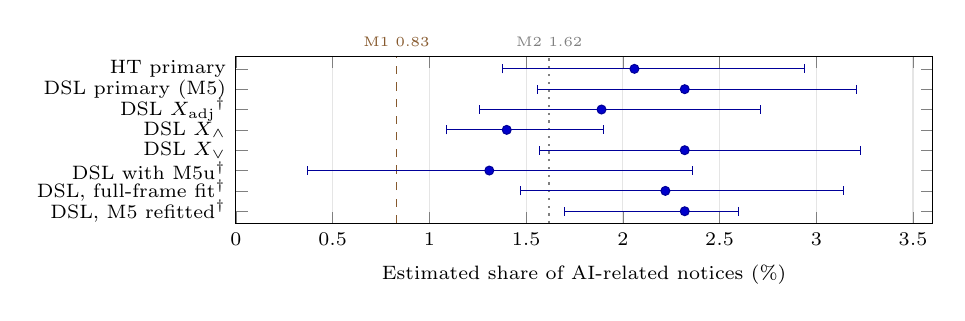
\begin{tikzpicture}
\begin{axis}[width=0.86\linewidth,height=3.7cm,xmin=0,xmax=3.6,ymin=0.4,ymax=8.6,
  ytick={1,...,8},
  yticklabels={DSL{,} M5 refitted$^\dagger$,DSL{,} full-frame fit$^\dagger$,DSL with M5u$^\dagger$,DSL $X_\vee$,DSL $X_\wedge$,DSL $X_{\mathrm{adj}}$$^\dagger$,DSL primary (M5),HT primary},
  tick label style={font=\scriptsize},label style={font=\scriptsize},
  xlabel={Estimated share of AI-related notices (\%)},xtick={0,0.5,...,3.5},
  xmajorgrids,major grid style={gray!20},clip=false]
\draw[dashed,brown!70!black] (axis cs:0.83,0.4) -- (axis cs:0.83,8.6) node[above,font=\tiny]{M1 0.83};
\draw[dotted,thick,gray] (axis cs:1.62,0.4) -- (axis cs:1.62,8.6) node[above,font=\tiny]{M2 1.62};
\addplot+[only marks,mark=*,mark size=1.6pt,color=blue!60!black,
  error bars/.cd,x dir=both,x explicit]
  coordinates {(2.06,8) += (0.88,0) -= (0.68,0)
               (2.32,7) += (0.89,0) -= (0.76,0)
               (1.89,6) += (0.82,0) -= (0.63,0)
               (1.40,5) += (0.50,0) -= (0.31,0)
               (2.32,4) += (0.91,0) -= (0.75,0)
               (1.31,3) += (1.05,0) -= (0.94,0)
               (2.22,2) += (0.92,0) -= (0.75,0)
               (2.32,1) += (0.28,0) -= (0.62,0)};
\end{axis}
\end{tikzpicture}
\caption{Design-based prevalence estimates with 95\% stratified bootstrap CIs, holding predictions fixed except for ``M5 refitted'' (refitted in each of 500 replicates). Full-frame fit: $\hat{g}$ cross-fitted over the frame. Vertical lines: frame flag rates (no sampling error). $^\dagger$Post hoc.}\label{fig:prev}
\end{figure}

\begin{table}[t]
\caption{Coefficient on AI-relatedness in a linear probability model of single bidding ($n=30{,}388$ notices with an eligible reported tender count; fixed effects for country, CPV division, procedure, buyer type, and quarter; log value). Percentage points with 95\% sandwich CIs unless noted. $^\dagger$Post hoc. $^\ddagger$Stratified bootstrap CI; sandwich SE 1,799.}\label{tab:reg}
\centering
\begin{tabular}{lrrr}
\toprule
Measurement of AI-relatedness & AI notices & $\hat\beta$ & 95\% CI or (SE) \\
\midrule
M1 English dictionary (plug-in) & 249 & $-1.7$ & [$-7.3$, 3.9] \\
M2 Multilingual dictionary (plug-in) & 470 & $-4.9$ & [$-8.9$, $-0.8$] \\
M4 Prototype similarity (plug-in) & 1,575 & $-1.2$ & [$-3.6$, 1.3] \\
M5 Embedding + LR (plug-in) & 31 & 2.7 & [$-12.2$, 17.6] \\
M6 TF-IDF + LR (plug-in) & 34 & $-11.4$ & [$-24.2$, 1.3] \\
Labelled notices only (weighted) & -- & 3.1 & [$-8.0$, 14.1] \\
DSL with M5 (pre-specified) & -- & $-123.5$ & [$-561$, 367]$^\ddagger$ \\
DSL with M5, full-frame cross-fitting$^\dagger$ & -- & $-119.0$ & (1,491.1) \\
DSL with M5, $X_{\mathrm{adj}}$ reference$^\dagger$ & -- & $-41.9$ & (177.1) \\
DSL with M5, $X_\wedge$ reference & -- & 6.1 & [$-6.8$, 18.9] \\
DSL with M5u$^\dagger$ & -- & $-24.9$ & [$-103.1$, 53.4] \\
\bottomrule
\end{tabular}
\end{table}

\subsection{AI-Relatedness and Single Bidding (H4)}
\label{sec:reg}
With plug-in indicators (Table~\ref{tab:reg}), M2 suggested that AI-related notices were 4.9 points less likely to report a single tender (CI $-8.9$ to $-0.8$), whereas all other plug-in CIs included zero. The pre-specified DSL estimate was uninformative ($\hat\beta=-123.5$ points, sandwich SE 1,799; bootstrap CI $-561$ to 367), and so was the full-frame cross-fitted estimate ($-119.0$ points, SE 1,491; post hoc). H4 was therefore not supported; the estimates did not establish the sign or size of the reference-defined association.

Post hoc diagnostics (Fig.~\ref{fig:diag}) locate the instability. For the pre-specified $\hat{g}$, $S$ (Eq.~\eqref{eq:schur}, for $N_R\hat{A}$, whose AI diagonal entry is 775.4) was 755.6 without controls and 705.7 with country fixed effects, where $\hat\beta$ was stable (21.8 and 19.8 points, SE 9.3 and 9.6), but $-95.9$ with full controls: $\hat{A}$ was indefinite and the denominator of $\hat\beta$ had crossed zero. The failure is thus a loss of information on $\beta$, not ill-conditioning alone: $\mathrm{cond}(\hat{A})$ was about $3\times10^6$ with full controls for every predictor, yet the SE with M5u was far smaller. The pseudo-outcomes reach 113.6 with M5 and 115.0 with the M2 indicator, produced by stratum-D positives with near-zero predictions, which push $S$ downward in sparse fixed-effect cells (Sect.~\ref{sec:design}); we did not decompose $S$ by cell. Open procedures contain no heavily weighted stratum-D positive (maximum pseudo-outcome 6.1), and there DSL with full controls was stable (1.0 points, SE 6.3); the plug-in M2 estimate was $-4.8$ points (CI $-9.9$ to 0.3). The restriction also aids construct validity: single-bid shares in $\mathcal{R}$ ranged from 38.6\% in open procedures to 93.9\% in negotiated procedures without prior call ($n=4{,}379$), where one tender is often inherent, so the no-control estimates are not read as associations. Precision also rose as fewer stratum-D positives remained in the reference ($X_{\mathrm{adj}}$, $X_\wedge$; Table~\ref{tab:reg}). In a synthetic check with a miscalibrated predictor (200 replications), 95\% sandwich intervals covered the true coefficient in only 85.5\% of replications, illustrating under-coverage under that design.


\begin{figure}[t]
\centering
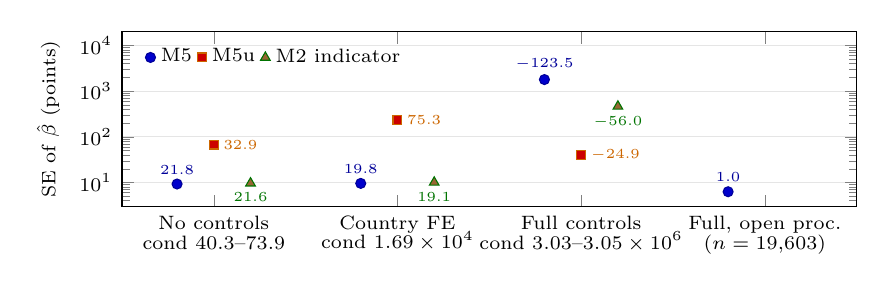
\begin{tikzpicture}
\begin{axis}[width=0.9\linewidth,height=3.8cm,ymode=log,ymin=3,ymax=2e4,
  xmin=0.5,xmax=4.5,xtick={1,2,3,4},
  xticklabels={{No controls\\[-1pt]cond 40.3--73.9},{Country FE\\[-1pt]cond $1.69\times10^4$},{Full controls\\[-1pt]cond $3.03$--$3.05\times10^6$},{Full, open proc.\\[-1pt]($n=19{,}603$)}},
  xticklabel style={align=center,font=\scriptsize},yticklabel style={font=\scriptsize},
  ylabel={SE of $\hat\beta$ (points)},label style={font=\scriptsize},
  ymajorgrids,major grid style={gray!20},
  legend style={font=\scriptsize,at={(0.02,0.97)},anchor=north west,draw=none,fill=none},legend columns=3,
  nodes near coords,point meta=explicit symbolic,
  every node near coord/.append style={font=\tiny}]
\addplot+[only marks,mark=*,mark size=1.8pt,color=blue!60!black,
  every node near coord/.append style={anchor=south}]
  coordinates {(0.8,9.3)[21.8] (1.8,9.6)[19.8] (2.8,1799.2)[$-$123.5] (3.8,6.3)[1.0]};
\addplot+[only marks,mark=square*,mark size=1.6pt,color=orange!80!black,
  every node near coord/.append style={anchor=west}]
  coordinates {(1,67.8)[32.9] (2,231.8)[75.3] (3,39.9)[$-$24.9]};
\addplot+[only marks,mark=triangle*,mark size=2pt,color=green!45!black,
  every node near coord/.append style={anchor=north}]
  coordinates {(1.2,9.7)[21.6] (2.2,10.1)[19.1] (3.2,466.8)[$-$56.0]};
\legend{M5,M5u,M2 indicator}
\end{axis}
\end{tikzpicture}
\caption{Post hoc diagnostics of the DSL regression coefficient by auxiliary predictor and control set (full: controls of Table~\ref{tab:reg}). Markers: SE of $\hat\beta$ (log scale); labels: $\hat\beta$ in points; cond: $\mathrm{cond}(\hat{A})$; M2 indicator: the stratum-constant M2 flag used as $\hat{g}$; open procedures: M5 only. For M5, $S>0$ in the first two control sets and $S<0$ with full controls.}\label{fig:diag}
\end{figure}

%======================================================================
\section{Discussion}
\subsubsection{Measurement.} The confirmatory result that survives multiplicity correction is H3; the excess over the English-dictionary flag rate remained positive under HT, full-frame cross-fitting, and every reference examined, but its magnitude rests on four stratum-D labels with a wide exact interval. The expanded multilingual dictionary achieved higher observed recall, although the contribution of language coverage could not be separated from differences in term selection \cite{gentzkow2019}. Under the primary reference, the recall of the English dictionary was not lower for non-English notices; the gap predicted by H1 appeared only under $X_\wedge$. The English--non-English recall gap of M4 is consistent with a language bias of its English prototypes, but our design cannot establish that cause.

\subsubsection{Why the supervised classifiers underperformed.} The ablation indicates that the low F1 was sensitive to both the inverse-probability training weights (about 115 in stratum D, at most two in the dictionary strata) and the fixed 0.5 threshold, and neither remedy reached the dictionaries. This concerns the classifiers tested at this label budget, not supervised measurement in general or a general superiority of dictionaries. Thresholded accuracy is also not what matters for DSL: M5 (lowest F1, highest AUPRC) gave the same SE as HT, whereas M5u (higher F1) gave a wider prevalence interval (1.31\%, CI 0.37--2.36\%); variance gains over HT require informative within-stratum predictions of the rare stratum-D positives \cite{egami2023,audinet2025}, which no predictor achieved.

\subsubsection{Downstream inference.} The CI of the plug-in multilingual-dictionary association excluded zero, but DSL did not establish its sign, and within open procedures its CI included zero. A significant coefficient obtained with a keyword indicator should not be read as evidence about AI procurement before its measurement error is quantified \cite{battaglia2025}. A few heavily weighted positives with near-zero predictions can make DSL regression unusable even when the prevalence estimate is stable; $S$ detects this directly and, unlike $\mathrm{cond}(\hat{A})$, is scale-invariant, so we recommend reporting it with DSL regressions. For monitoring, the results favour multilingual screening plus a labelled probability sample that spends more of its budget on the unflagged stratum, where most uncertainty lies.

%======================================================================
\section{Limitations}
No independent human expert validated the reference labels; the LLM checks assess cross-model agreement and label sensitivity only, and the three models may share errors. The label sensitivity analysis is not exhaustive (e.g., the 33 missing secondary labels and joint recodings of the four stratum-D positives were not stress-tested). Neither cross-fitting variant makes fold predictors exactly independent of the inclusion indicators; the primary intervals hold predictors fixed and omit the finite-population correction, and sandwich intervals under-covered in our synthetic check. The weight and threshold ablation covers M5 only, and no HT moment regression ($\hat{g}\equiv0$) was estimated. The frame covers two CPV divisions in TED, mostly above EU thresholds. In the regression, lot structure and selection into $\mathcal{R}$ are not modelled, the controls omit buyer experience and supplier history, and all associations are non-causal. The dictionaries were written by the authors and may contain translation errors, the stratification makes the precision for other methods design-dependent, and the primary experiments used one compact multilingual encoder, with one alternative encoder examined post hoc, and linear classifiers.

%======================================================================
\section{Conclusion}
In 54,160 multilingual TED award notices, analysed with a pre-specified stratified reference sample and design-based estimation, a multilingual dictionary roughly doubled the observed recall of an English keyword list, which flagged notices at about one third of the estimated reference-defined prevalence; the direction of this gap was robust to the estimator, the cross-fitting scheme, and contested labels, but its size was not. An apparent negative association with single bidding under plug-in measurement could not be confirmed after adjustment relative to the LLM reference labels, because the DSL moment matrix became indefinite under the full controls. Future work should obtain expert labels for the influential cases, sample the unflagged stratum further, use survey-specific variance estimation, test fine-tuned multilingual classifiers, and extend the analysis to national systems such as the Korean KONEPS.

\begin{credits}
\subsubsection{\ackname} The authors thank the Publications Office of the European Union for providing open access to TED notices. This research received no specific grant from any funding agency in the public, commercial, or not-for-profit sectors.

\subsubsection{Author contributions.} Jinkyu Lee designed the study, carried out the experiments and the analysis, and wrote the manuscript. Chang Soo Sung reviewed the manuscript and provided feedback for its revision.

\subsubsection{Data and code availability.} Code, prompts, dictionaries, the analysis plan and its amendment, annotation logs, and notice-level derived data (notice identifiers, scores, and labels, without notice texts) are available at \url{https://github.com/leejinkyu0612-hue/ted-ai-procurement-measurement}.

\subsubsection{Use of generative AI.} Two LLMs (Claude Haiku 5.5 and Gemini 2.5 Flash-Lite, accessed through OpenRouter) were used as research instruments to annotate the reference sample, as described in Sect.~3.2. In addition, the authors used ChatGPT (OpenAI) and Claude (Anthropic) to assist with literature search, drafting, language editing, code generation, and structured internal review. All reported numbers are taken from logged outputs of the released code, and all references were checked against their DOI or publisher pages. The authors reviewed all content and take full responsibility for the publication.

\subsubsection{\discintname} Jinkyu Lee is the founder and CEO of HappyAI; the authors declare no other competing interests.
\end{credits}

\bibliographystyle{splncs04}
\bibliography{refs}
\end{document}
